\chapter{Кинетический момент системы в абсолютном движении. Теорема об
изменении кинетического момента системы в относительном движении по
отношению к центру масс. Дифференциальные уравнения плоского движения
твердого тела.}

Моментом количества движения системы материальных точек \( \vec{K}_O \)
относительно некоторого центра \( O \) называется векторная сумма моментов
количества движения отдельных точек этой системы относительно того же центра
\( O \):
\[
    \vec{K}_O = \sum \vec{k}_{O_j} = \sum \vec{r}_j\times m_j\vec{v}_j.
\]
 
Моментом количества движения системы материальных точек \( K_z \) относительно
какой-либо оси \( Oz \), проходящей через центр \( O \), называется проекция
вектора количества движения \( \vec{K}_O \) на эту ось:
\[
    K_z = K_O\cos\alpha.
\]

\section{Теорема об изменении кинетического момента механической системы при ее
движении вокруг неподвижного центра}
Полная производная по времени от вектора кинетического момента механической
системы относительно некоторого неподвижного центра \( O \) по величине и
направлению равна главному моменту внешних сил, приложенных к механической
системе, определенному относительно того же центра:
\[
    \der{\vec{K}_O}{t} = \vec{M}^e_O,
\]
где
\[
    \vec{M}^e_O = \sum_{k=1}^N \vec{m}^e_{O_k} = 
    \sum_{k=1}^N \vec{r}_k\times\vec{F}^e_k \text{ --}
\]
главный момент всех внешних сил относительно центра \( O \).

При  решении  задач, в которых рассматриваются тела, вращающиеся вокруг
неподвижной оси, используют теорему об изменении кинетического момента
относительно неподвижной оси:
\[
    \der{K_z}{t} = M^e_z = \sum_{k=1}^N m^e_{z_k}.
\]
 
\section{Следствия из теоремы об изменении кинетического момента}
\begin{enumerate}
    \item Если главный момент всех внешних сил относительно некоторого
    неподвижного центра равен нулю, то кинетический момент механической системы
    относительно этого центра остается неизменным.
    \item Если главный момент всех внешних сил относительно некоторой
    неподвижной оси равен нулю, то кинетический момент механической системы
    относительно этой оси остается неизменным.
\end{enumerate}

Дифференциальные уравнения движения тела могут быть получены при помощи теоремы
о движении центра масс и теоремы об изменении кинетического момента.

Получим эти уравнения для основных видов движения тела -- поступательного,
вращательного и плоского.

При поступательном движении все точки тела движутся одинаково. По этой причине,
определив движение какой-то одной точки тела, одновременно получаем все данные и
о движении остальных точек. В качестве такой определяющей точки выберем центр
масс тела, так как именно для него известно правило составления дифференциальных
уравнений движения, устанавливаемое теоремой о движении центра масс.

Дифференциальные уравнения движения центра масс
\[
    m\ddot{x} = \sum_{k=1}^N F^e_{x_k},
    \quad m\ddot{y} = \sum_{k=1}^N F^e_{y_k},
    \quad m\ddot{z} = \sum_{k=1}^N F^e_{z_k}.
\] 
одновременно служат дифференциальными уравнениями поступательного движения тела.
В этих уравнениях индекс центра масс опущен, так как теперь \( (x, y, z) \) --
координаты любой точки тела.

\begin{minipage}{.4\textwidth}
    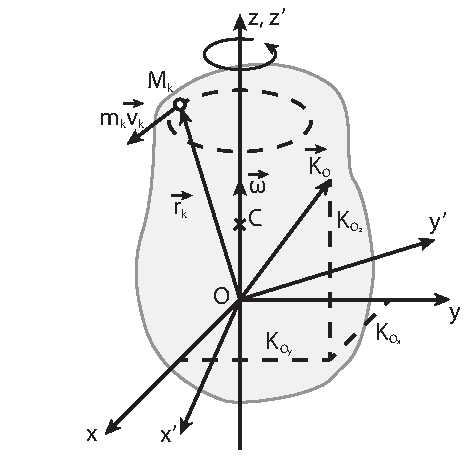
\includegraphics[width=\textwidth]{50_01}
\end{minipage}\hfill
\begin{minipage}{.55\textwidth}
Дифференциальное уравнение вращательного движения получим, воспользовавшись
теоремой об изменении кинетического момента относительно оси вращения тела.
Совмещая ось вращения с координатной осью (см. рис.), запишем
\[
    \der{K_z}{t} = M^e_z.
\]
 
Подставляя сюда равенства
\[
    K_z = I_z\omega_z = I_z\dot{\phi} \text{ и }
    M^e_z = \sum_{k=1}^N m^e_{z_k},
\]
\end{minipage}
получаем дифференциальное уравнение вращательного движения:
\[
    I_z\ddot{\phi} = \sum_{k=1}^N m^e_{z_k}.
\]
 
Направление отсчета угла поворота удобно совместить с направлением вращения
тела. Тогда правило знаков при вычислении моментов внешних сил, сумма которых
стоит в правой части уравнения, будет такое: момент положителен, если направлен
в сторону вращения тела; момент отрицателен, если направлен против вращения
тела.

\newpage
